%; whizzy chapter
% -initex iniptex -latex platex -format platex -bibtex jbibtex -fmt fmt
% $B0J>e(B whizzytex $B$r;HMQ$9$k>l9g$N@_Dj!#(B

%     Tokyo Debian Meeting resources
%     Copyright (C) 2010 Junichi Uekawa

%     This program is free software; you can redistribute it and/or modify
%     it under the terms of the GNU General Public License as published by
%     the Free Software Foundation; either version 2 of the License, or
%     (at your option) any later version.

%     This program is distributed in the hope that it will be useful,
%     but WITHOUT ANY WARRANTY; without even the implied warranty of
%     MERCHANTABILITY or FITNESS FOR A PARTICULAR PURPOSE.  See the
%     GNU General Public License for more details.

%     You should have received a copy of the GNU General Public License
%     along with this program; if not, write to the Free Software
%     Foundation, Inc., 51 Franklin St, Fifth Floor, Boston, MA  02110-1301 USA

%  preview (shell-command (concat "evince " (replace-regexp-in-string "tex$" "pdf"(buffer-file-name)) "&"))
% $B2hA|%U%!%$%k$r=hM}$9$k$?$a$K$O(Bebb$B$rMxMQ$7$F(Bboundingbox$B$r:n@.!#(B
%(shell-command "cd image201011; ebb *.jpg")

%%$B$3$3$+$i%X%C%@3+;O!#(B

\documentclass[mingoth,a4paper]{jsarticle}
\usepackage{monthlyreport}
\usepackage{wrapfig}

% $BF|IU$rDj5A$9$k!"Kh7nJQ$o$j$^$9!#(B
\newcommand{\debmtgyear}{2010}
\newcommand{\debmtgmonth}{11}
\newcommand{\debmtgdate}{20}
% (+ (* (- 2010 2005) 12) 10) started from zero
\newcommand{\debmtgnumber}{70}

\begin{document}

\begin{titlepage}
\thispagestyle{empty}
% $B%?%$%H%k%Z!<%8(B:$BJT=8I,MW$JItJ,$O:G=i$N%^%/%m$KHt$P$9$3$H(B

\vspace*{-2cm}
$BBh(B\debmtgnumber{}$B2s(B $BEl5~%(%j%"(B Debian $BJY6/2q;qNA(B\\
\hspace*{-2cm}
\includegraphics[width=210mm]{image201003/debsen.eps}\\
\hfill{}\debmtgyear{}$BG/(B\debmtgmonth{}$B7n(B\debmtgdate{}$BF|(B

% $B$3$3$O%"%C%W%G!<%H$9$k$3$H(B
\rotatebox{10}{\fontsize{32}{32} {\gt $BFC=8(B: $B%F%l%S$r8+$?$j(B}}

\vspace*{-2cm}
\hfill{}
\includegraphics[height=6cm]{image200502/openlogo-nd.eps}
\end{titlepage}

\dancersection{Introduction}{$B>e@n(B $B=c0l(B}

\begin{multicols}{2}
 

 $B:#7n$N(BDebian$BJY6/2q$X$h$&$3$=!#$3$l$+$i(BDebian$B$N@$3&$K$"$7$rF'$_F~$l$k$H(B
 $B$$$&J}$b!"$9$G$K$I$C$W$j$H$D$+$C$F$$$k$H$$$&J}$b!"7n$K0l2s(BDebian$B$K$D$$(B
 $B$F8l$j$^$;$s$+!)(B

 Debian$BJY6/2q$NL\E*$O2<5-$G$9!#(B

 \begin{itemize}
 \item \underline{Debian Developer} ($B3+H/<T(B)$B$N0i@.!#(B
 \item $BF|K\8l$G$N!V(B\underline{$B3+H/$K4X$9$k>pJs(B}$B!W$r@0M}$7$F$^$H$a!"%"%C%W%G!<%H$9$k!#(B
 \item \underline{$B>l(B}$B$NDs6!!#(B
 \begin{itemize}
  \item $BIaCJ$P$i$P$i$J>l=j$K$$$k?M!9$,(B face-to-face $B$G=P2q$($k>l$rDs6!(B
	$B$9$k!#(B
  \item Debian $B$N$?$a$K$J$k$3$H$r8l$k>l$rDs6!$9$k!#(B
  \item Debian$B$K$D$$$F8l$k>l$rDs6!$9$k!#(B
 \end{itemize}
 \end{itemize}		

 Debian$B$NJY6/2q$H$$$&$3$H$G5f6KE*$K$O;22C<TA40w$,(BDebian Package$B$r$,$j$,$j(B
 $B$H:n$k%9!<%Q!<%O%C%+!<$K$J$C$?;Q$rLQA[$7$F$$$^$9!#>pJs$N6&M-!&3hMQ$rDL$7(B
 $B$F(B Debian$B$N:#8e$NG=F0E*$JE83+$X$NEZBf$H$7$F!"!V>l!W$H$7$F$N6u4V$rDs6!$9(B
 $B$k$N$,L\E*$G$9!#(B

\end{multicols}

\newpage

\begin{minipage}[b]{0.2\hsize}
 \definecolor{titleback}{gray}{0.9}
 \colorbox{titleback}{\rotatebox{90}{\fontsize{80}{80} {\gt $B%G%S%"%sJY6/2q(B} }}
\end{minipage}
\begin{minipage}[b]{0.8\hsize}
\hrule
\vspace{2mm}
\hrule
\begin{multicols}{2}
\tableofcontents
\end{multicols}
\vspace{2mm}
\hrule
\end{minipage}

\dancersection{$B;vA02]Bj(B}{$B>e@n(B $B=c0l(B}

$B:#2s$N;vA02]Bj$O0J2<$G$9(B:

\begin{itemize}
 \item xxx
\end{itemize}

$B$3$N2]Bj$KBP$7$FDs=P$$$?$@$$$?FbMF$O0J2<$G$9!#(B

% \begin{prework}{ ����(yy\_y\_ja\_jp) }
���ޤ���������ǤϤʤ��Ǥ���... �긵�Υ�åץȥåפǤ� /boot �ˤ� ext2
 ����¾�ˤ� ext3���Ƕ�ȤäƤ���ǥ����ȥåפǤ� /boot �ˤ� ext3 ����¾
 �ˤ� LVM ��� ext4 ��ȤäƤ��ޤ���
\end{prework}

\begin{prework}{ �����ϥ� }
�ǥե���Ȥ�ext3����
�����ǥե���ȤΤޤޡ�
(NTFS���VM���᡼�����ext3�⤢�뤱��)
\end{prework}

\begin{prework}{ yos.takahashi }
ext3/4���˻ȤäƤޤ���ext3�Υǡ�������١����ˤĤ�������Linux2011ǯ1���˼�ɮ���ޤ�����
\end{prework}

\begin{prework}{ MATOHARA }
����inode �ϳ���������Ƥ���inode ��ưŪ�˳�����Ƥ���XFS �����򤹤뤳
 �Ȥ�¿���Ǥ���NILFS �Ͼ�����Ƥߤ��ΤǤ�����mount ���˰ʲ��Τ褦�ʥ��
 ���������ФƤޤ��ݤ��ʤȻפ��ޤ�����
\begin{commandline}
$ sudo mount /dev/sdb1 /mnt
mount.nilfs2: WARNING! - The NILFS on-disk format may change at any time.
mount.nilfs2: WARNING! - Do not place critical data on a NILFS filesystem. 
\end{commandline}
����¾NotePC �Ǥ�dm-crypt �ξ�˥ե����륷���ƥ���֤��ưŹ沽�����ꡢ
 eCryptfs �ǰŹ沽�����ꤷ�Ƥ��ޤ����񤭹��߻���CPU �򤫤ʤ���񤷤ޤ��ġ�
\end{prework}

\begin{prework}{ ��ޤ� }
��ext2-$>$reiserfs-$>$jfs-$>$xfs-$>$reiserfs-$>$ext3�ȻȤäƤ��ޤ�����

����:
\begin{itemize}
 \item reiserfs: ���ե������¿���ե�����Υ������������ӥ��Ӥ��Ƥ��ɤ���
       �����������դȤ����ⵤ�������θ�μ�žȬ�ݥ����ɤˡ�����
 \item jfs: ����v1.0��̾��ä�IBM���ꥨ�ʥ��������ˤ�xfs��ƨ��
 \item xfs: fsck==true�˴�ư����������ǯ�Ȥä���ΤΥޥ�����Ĵ����0byte
       �ե��������������Ѥ���줺ƨ����
\end{itemize}
������reiser4��Ķ���Ԥ��뤦���ˤ��줬�����ʤäơ����ext3�˸��경��htree�����ä������⤦Ŵ�Ĥʤ鲿�Ǥ⤤���Ǥ��������Ȥ����Ĥ�nilfs�ʤɤ˼��Ф��Ƥ��ޤ���ext3�������noatime���٤Ǥ����������aufs���碌�Ƽ�ʬ���Ȥ��Ȥ� *strap �Ķ��򥯥����˥󥰤��Ƥ��ޤ����¸����ƥ��Ȥ������Ǥ�����Ǥ���USB�����ư�Ǥ�ͭ�ѡ�

���LVM�ǤϤʤ�MD��Ȥäƾ�Ĺ���ܥХå����åפ򤷤Ƥ��ޤ���
 MD(sda,sdb,sdc)�ǹ��ۤ����̾��MD(����)�Dz�ư���Хå����åפλ���
 attach/detach�򤹤롣�֥��å���٥�ʤΤǥꥫ�Х��FSǤ���Ǥ��������̤�
 �������¾����ˡ���ʤ�������
\end{prework}

\begin{prework}{ henrich }
�ȤäƤ���֤�NTFS��Ĺ���󤸤�ʤ��Ǥ����͡����졣
�����Ρ����Ѥο������ǥ�������ext4�ǥե����ޥåȤ��ޤ����������㤤��Ƚ��ʤ��Ȥ����������Ƥ��ޤ���
\end{prework}

\begin{prework}{ emasaka }
�Ĥ뤷��FS��ȤäƤޤ�
\end{prework}

\begin{prework}{ �ܾ� }
ext3����Ѥ��Ƥ��ޤ����ä��Ѥ�ä����ȤϤ��Ƥ��ޤ���
FS����ʤ��Ǥ������Ƕ�Lenny��2TB��HDD��Ȥä���parted�äƤλȤ��ƶä��ޤ�����
\end{prework}

\begin{prework}{ ����@������ }
���������Ū�˳��Ѥ��Ƥ���ե����륷���ƥ��ReiserFS�Ǥ���
�Ż��ǻȤäƤ�Ķ���ext3�Ǥ�����ext3���Ÿ������ǥ��㡼�ʥ뤬
����Ʋ��Ǥ������ηи��ʸŤ������ͥ�Ǥ���...�ˤ����ꡢ
���ޤ꿮�Ѥ��Ƥ��ޤ���
�����ReiserFS�Ķ��ǤϤ���ޤǤνꤤ���ʤ��Ÿ����ڤä��ꡢ
�Ƥ�HDD�����줫�����ꤷ�Ƥ��ﳲ����ä��и���̵���Τǡ�
��³Ū�˻ȤäƤ��ޤ���
��ǯ����ReiserFS�Υᥤ��ȯ��(Hans Reiser)�����ᤵ��Ƥ��ޤ������ƥʥ󥹤��ۤ��Ƥ��ޤ�����
�����������θ��ReiserFS��¾�γ�ȯ�Ԥˤ���³�����ݼ餵��Ƥ���Τǡ��¿����ޤ�����
\end{prework}

\begin{prework}{ nozzy123nozzy }
\begin{enumerate}
 \item LVM�ˤĤ��Ƥϡ�CentOS5.5��Ƴ�������Τ��Τޤޤ����Ѥ��Ƥޤ�����
       ���������ƥब��äƤ���Volume̾�ϥǥե���Ȥ�����ȡʼºݤˤ�
       kickstart�ˤơˤ��ѹ����ƻȤäƤޤ����ʾ㳲���Υ���١����˺��뤿
       ���
\item ext3�ˤĤ��Ƥϡ�debian-sid�����Τޤ޻��ꤷ�Ƥ����Τ򤽤Τޤ޻Ȥ�
      �Ƥ����ꤷ�ޤ���relatime, noatime ���餤�Ͼ����ɲä��Ƥߤ����ʡ���
      �ϻפäƤޤ���
\end{enumerate}
\end{prework}

\begin{prework}{ �ޤ��������ؤ� }
\begin{itemize}
 \item Debian�Ǥ��ä˶Ťä����Ȥ�����ext3��ȤäƤޤ������ۥޥ����qcow2
       ���᡼���ǥ��������ѻ��ʳ��ϡ�LVM�ϻȤäƤޤ���
 \item �����ǰ����ü�ʤΤϡ��������DHCP�������Ѥ�Armadillo-J�ǻȤäƤ�
       ��JFFS�Ǥ����ǥե���ȤΥե����०�����Ǥϥ�֡��Ȥ�����������
       �ƽ��������Ƥ��ޤ��Τǡ�RAM�ΰ�˽񤭤��ߡ��Ÿ��ڤäƤ�ä��ʤ�
       ���������Ǥ���Debian��udhcp�Υ������ѥå���������ӥ�ɤ��ƻȤäƤޤ���
       \footnote{\url{http://d.hatena.ne.jp/mkouhei/20080601/1212330630}}
 \item ��Debian���ߤǡ���ʬ����ǰ��֥ۥåȤʤΤ�palm webOS�Ǥ��������Ubuntu��
       �������ޥ���������Τ餷���ΤǤ�����/etc/mtab�򸫤��35�Ԥ⤢�ꡢ
       ���ʤ����֤ʹ����Ǥ��͡�
\end{itemize}
\end{prework}

\dancersection{$B:G6a$N(BDebian$B4XO"$N%_!<%F%#%s%0Js9p(B}{$B4d>>?.MN(B}
\subsection{$BEl5~%(%j%"(BDebian$BJY6/2q(B69$B2sL\Js9p(B}
% (query-replace-regexp "<.*?>" "")
% (query-replace-regexp "^[	 ]\+" "")

%-------------------------------------------------------------------------------
\dancersection{ext4 $B%U%!%$%k%7%9%F%`$r(BDebian$B$G3hMQ$7$F$_$k(B}{$B>e@n(B $B=c0l(B}
%-------------------------------------------------------------------------------
\index{ext4}

ext4 $B%U%!%$%k%7%9%F%`$O(B Linux $B$G9-$/;H$o$l$F$$$k(B ext3 $B$N8e7Q%U%!%$%k%7%9(B
$B%F%`$H$7$FEP>l$7$?%U%!%$%k%7%9%F%`$G$9!#FCD'$H$7$F$O!"(Bext3 $B$HF1$8$/%8%c!<(B
$B%J%j%s%05!G=$r$b$A!"%G!<%?NN0h$r%V%m%C%/C10L$G$O$J$/%(%/%9%F%s%H(B($B0lO"$NNN(B
$B0h(B)$B$G3NJ]$7$F$$$k$3$H!#(B32$B%S%C%H$+$i(B48$B%S%C%H$K$J$C$?$N$G!"%U%!%$%k%7%9%F%`(B
$B%5%$%:$,(Bext3 $B$N@)8B$r1[$($F$$$k!#(Batime$B$J$I$,IC$h$j:Y$+$$;~4V$G$o$+$k$h$&(B
$B$K$J$k!"$J$I$G$9!#(B\cite{ext42007,ext42008}

\subsection{ext4 $B%U%!%$%k%7%9%F%`$r:n$C$F$_$k(B}

$B$=$l$G$O!"(Bext4$B%U%!%$%k%7%9%F%`$r:n$C$F$_$^$7$g$&!#<B$ODL>o$N(Bext3$B%U%!%$%k(B
$B%7%9%F%`$r$=$N$^$^(Bext4$B$H$7$F%^%&%s%H$9$k$3$H$b$G$-$k$h$&$G$9!#$=$&$9$k$H=y!9$K(B
$B%U%!%$%k$,=q$-49$($k$?$S$K(Bextent$B%Y!<%9$K$J$C$?$j$9$k$h$&$G$9!#(B
$B$?$@!"%U%!%$%k%7%9%F%`A4BN$N%Q%i%a!<%?$,(Bext4$BMQ$G$O$J$$$N$G!"%U%!%$%k%7%9(B
$B%F%`$r$$$A$+$i:n@.$9$k$N$,$h$$$G$7$g$&!#(B

$B%"%m%1!<%?$N%"%k%4%j%:%`$b2~A1$5$l$F$$$k$N$G>.$5$J%U%!%$%k$N%"%m%1!<%7%g(B
$B%s$b2~A1$7$F$$$k$h$&$G$9$N$G!"4{B8$N%U%!%$%k%7%9%F%`$NFbMF$r%P%C%/%"%C%W(B
$B$7$F%j%9%H%"$9$k$N$,$h$$$N$G$O$J$$$G$7$g$&$+!#(B

ext4 $B$r;H$&$K$O==J,?7$7$$(B e2fsprogs $B$H==J,$"$?$i$7$$(BLinux Kernel $B$,$"$l$P(B
$B$h$$$G$9!#(BDebian 5.0 (lenny) $B$N;~E@$GI,MW$J%Q%C%1!<%8$O$=$m$C$F$$$k$h$&$G$9!#(B

\begin{commandline}
 $ sudo lvcreate -L 1G -n lvext4 vghoge
  Logical volume "lvext4" created
 $ sudo mount /dev/vghoge/lvext4 /mnt/
 $ mount -v 
 /dev/mapper/vghoge-lvext4 on /mnt type ext4 (rw)
 $ df -h /mnt/
 Filesystem          $B%5%$%:(B  $B;HMQ(B  $B;D$j(B $B;HMQ(B% $B%^%&%s%H0LCV(B
 /dev/mapper/vghoge-lvext4
                     1008M   34M  924M   4% /mnt
 $ df -T /mnt/ 
 Filesystem    Type   1K-$B%V%m%C%/(B    $B;HMQ(B   $B;HMQ2D(B $B;HMQ(B% $B%^%&%s%H0LCV(B
 /dev/mapper/vghoge-lvext4
              ext4     1032088     34052    945608   4% /mnt
 $ df -i /mnt/
 Filesystem            I$B%N!<%I(B  I$B;HMQ(B   I$B;D$j(B I$B;HMQ(B% $B%^%&%s%H0LCV(B
 /dev/mapper/vghoge-lvext4
                       65536      11   65525    1% /mnt
\end{commandline}

\begin{thebibliography}{0}
 \bibitem{ext42007} A. Mathur, M. Cao, S. Bhattacharya, A. Dilger, A. Tomas, and
 L. Vivier. "The new ext4 filesystem: current status and future plans,"
 Linux Symposium. 2007

 \bibitem{ext42008}  A. Kumar K. V., M. Cao, J. R. Santos, and A. Dilger. "Ext4 block and inode allocator improvements," Linux Symposium, Vol 1. 2008.

\end{thebibliography}

%-------------------------------------------------------------------------------
\dancersection{NILFS$B$r(BDebian$B$G3hMQ$7$F$_$k(B}{$B;3ED(B $BBY;q(B}
%-------------------------------------------------------------------------------
\index{NILFS}

\subsection{NILFS$B$C$F$I$s$J%U%!%$%k%7%9%F%`(B?}
\subsection{$B%$%s%9%H!<%kJ}K!(B}

Debian$B$G%$%s%9%H!<%k$9$kJ}K!(B

\subsection{$B%^%&%s%H!&(Bfsck}


\subsection{$B%P%C%/%"%C%WMQ$N%U%!%$%k%7%9%F%`$H$7$F;H$C$F$_$k(B}

%-------------------------------------------------------------------------------
\dancersection{Btrfs$B$r(BDebian$B$G3hMQ$7$F$_$k(B}{$BNkLZ(B $B?rJ8(B}
%-------------------------------------------------------------------------------
\index{Btrfs}

\subsection{Btrfs$B$C$F$I$s$J%U%!%$%k%7%9%F%`(B?}
Btrfs $B$O!"(BLinux kernel $B$N(B 2.6.29 $B$+$i(B kernel $B$N%j%j!<%9$K$b4^$^$l$k$h$&$K$J$C$?!"?7$7$$%3%T!<%*%s%i%$%H7A<0$N%U%!%$%k%7%9%F%`$G$"$j!"%U%)!<%k%H%H%l%i%s%H$d=$I|5!G=!"MF0W$J4IM}5!G=$J$I$,Hw$o$C$F$$$^$9!#(BZFS $B$N1F6A$r<u$1$F$$$k$H8@$o$l$F$*$j!"(BOracle $B$N(B Chris Mason $B$K$h$j(B GPL $B$G3+H/$,$9$9$a$i$l$F$$$^$9!#(B
$B8=:_$O$^$@3+H/Cf$N>uBV$K$"$j$^$9!#(B

$B$J$*!":#2s$O(B Debian Squeeze/Sid $B$r;HMQ$7$F2r@b$7$^$9$,!"(BSqueeze/Sid $B$N(B README $B$K$*$$$F$b!"$^$@8=;~E@$G$O%Y%s%A%^!<%/$H%l%S%e!<0J30$K;HMQ$9$k$J$H$NCm0U=q$-$,$"$j$^$7$?!#(B
\begin{commandline}
$ cat /usr/share/doc/btrfs-tools/README.Debian
btrfs-tools for Debian
----------------------

WARNING: Btrfs is under heavy development, and is not suitable for any uses
other than benchmarking and review.

 -- Daniel Baumann <daniel@debian.org>  Sun, 29 Jul 2007 12:19:00 +0200
\end{commandline}


\subsection{Debian$B$G%$%s%9%H!<%k$9$kJ}K!(B}
Debian $B$G(B Btrfs $B$r;HMQ$9$k<j=g$O!"(Bbtrfs-tools $B%Q%C%1!<%8$r%$%s%9%H!<%k$9$k$@$1$K$J$j$^$9!#(B
\begin{commandline}
$ sudo apt-get install btrfs-tools
\end{commandline}


\subsection{$B%U%)!<%^%C%H!&%^%&%s%H!&(Bbtrfsck}

$B%U%)!<%^%C%H$O(B mkfs.btrfs $B$G9T$($^$9!#(B
\begin{commandline}
# mkfs.btrfs /dev/sda

WARNING! - Btrfs Btrfs v0.19 IS EXPERIMENTAL
WARNING! - see http://btrfs.wiki.kernel.org before using

fs created label (null) on /dev/sda
        nodesize 4096 leafsize 4096 sectorsize 4096 size 500.00MB
Btrfs Btrfs v0.19
\end{commandline}

$B%^%&%s%H$bDL>oDL$j!"(Bmount $B$r;HMQ$G$-$^$9!#(B
\begin{commandline}
# mkdir /mnt/btrfs1
# mount /dev/sda /mnt/btrfs1
# df -T
Filesystem    Type   1K-blocks      Used Available Use% Mounted on
/dev/sde1     ext3    19272572   2833388  15460192  16% /
tmpfs        tmpfs      517260         0    517260   0% /lib/init/rw
udev         tmpfs      512936       100    512836   1% /dev
tmpfs        tmpfs      517260         0    517260   0% /dev/shm
/dev/sda     btrfs      512000    205092    306908  41% /mnt/btrfs1
\end{commandline}

$B$3$3$G;n$7$K%U%!%$%k$r%3%T!<$7$F$_$k$H!"<!$N$h$&$K%3%T!<%*%s%i%$%H$N$*$+$2$G9bB.$J%3%T!<$,$5$l$F$$$k$3$H$,$o$+$j$^$9!#(B
\begin{commandline}
# ls -al /mnt/btrfs1/
total 102408
dr-xr-xr-x 1 root root         8 Nov 17 04:14 .
drwxr-xr-x 3 root root      4096 Nov 17 04:01 ..
-rw-r--r-- 1 root root 104857600 Nov 17 04:03 data
# time cp /mnt/btrfs1/data  /mnt/btrfs1/data-copy

real    0m0.731s
user    0m0.000s
sys     0m0.556s
# ls -al /mnt/btrfs1/
total 116584
dr-xr-xr-x 1 root root        26 Nov 17 04:14 .
drwxr-xr-x 3 root root      4096 Nov 17 04:01 ..
-rw-r--r-- 1 root root 104857600 Nov 17 04:03 data
-rw-r--r-- 1 root root 104857600 Nov 17 04:14 data-copy
\end{commandline}

$B%I%-%e%a%s%H$K$O(B fsck $B$O$^$@40A4$K$O<BAu$5$l$F$*$i$:!"%"%s%^%&%s%H$5$l$?>uBV$G(BFS$B%(%/%9%F%s%H%D%j!<$N%A%'%C%/$N$_$,<BAu$5$l$F$$$k!"$H5-:\$5$l$F$$$^$7$?$,!"<B:]$K<B9T$7$?$H$3$m$G$O%^%&%s%H>uBV$G$"$C$F$b<B9T$G$-$^$7$?!#(B
$B$J$*!"!V(B-a$B!W%*%W%7%g%s$,<BAu$5$l$F$$$J$$$?$a8=;~E@$G$O(B fsck.btrfs $B$X$N%7%s%\%j%C%/%j%s%/$OB8:_$;$:!"(Bbtrfsck $B$rD>@\<B9T$9$kI,MW$,$"$j$^$9!#(B
\begin{commandline}
# btrfsck /dev/sda
found 210018304 bytes used err is 0
total csum bytes: 204800
total tree bytes: 303104
total fs tree bytes: 8192
btree space waste bytes: 74736
file data blocks allocated: 209715200
 referenced 209715200
Btrfs Btrfs v0.19
\end{commandline}

\subsection{$BJ#?t$N%G%#%9%/$r;HMQ$7$F$_$k(B}

Btrfs $B$G$OJ#?t$N%G%#%9%/$NB+$M$F;HMQ$9$k$3$H$b$G$-$^$9!#$3$3$G$O@h$[$I:n@.$7$?(B /dev/sda $B$K(B /dev/sdb $B$rDI2C$7$F$_$^$9!#(Bbtrfs device add $B$G4JC1$KDI2C$G$-$^$9!#(Bdf $B$GDI2C$7$?J,$NMFNL$,A}$($F$$$k$3$H$,3NG'$G$-$^$9!#(B
\begin{commandline}
# df
Filesystem           1K-blocks      Used Available Use% Mounted on
/dev/sde1             19272572   3414148  14879432  19% /
tmpfs                   517260         0    517260   0% /lib/init/rw
udev                    512936       100    512836   1% /dev
tmpfs                   517260         0    517260   0% /dev/shm
/dev/sda                512000        28    511972   1% /mnt/btrfs1
# btrfs device add /dev/sdb /mnt/btrfs1/
# df
Filesystem           1K-blocks      Used Available Use% Mounted on
/dev/sde1             19272572   3414148  14879432  19% /
tmpfs                   517260         0    517260   0% /lib/init/rw
udev                    512936       100    512836   1% /dev
tmpfs                   517260         0    517260   0% /dev/shm
/dev/sda               1024000        28   1023972   1% /mnt/btrfs1
\end{commandline}

$B0J2<$N$h$&$K%U%)!<%^%C%H;~$+$iJ#?t$N%G%#%9%/$rB+$M$F%U%)!<%^%C%H$9$k$3$H$b$G$-$^$9!#(B
\begin{commandline}
# mkfs.btrfs /dev/sda /dev/sdb

WARNING! - Btrfs Btrfs v0.19 IS EXPERIMENTAL
WARNING! - see http://btrfs.wiki.kernel.org before using

adding device /dev/sdb id 2
fs created label (null) on /dev/sda
        nodesize 4096 leafsize 4096 sectorsize 4096 size 1000.00MB
Btrfs Btrfs v0.19
# mount /dev/sda /mnt/btrfs1
# df
Filesystem           1K-blocks      Used Available Use% Mounted on
/dev/sde1             19272572   3414152  14879428  19% /
tmpfs                   517260         0    517260   0% /lib/init/rw
udev                    512936       100    512836   1% /dev
tmpfs                   517260         0    517260   0% /dev/shm
/dev/sda               1024000        28   1023972   1% /mnt/btrfs1
\end{commandline}


\subsection{$B%P%C%/%"%C%WMQ$N%U%!%$%k%7%9%F%`$H$7$F;H$C$F$_$k(B}

$B$^$:$O!"%5%V%\%j%e!<%`$r:n@.$7$^$9!#(B
\begin{commandline}
# btrfs subvolume create /mnt/btrfs1/subvolume
Create subvolume '/mnt/btrfs1/subvolume'
\end{commandline}

$B$3$N:n@.$7$?%5%V%\%j%e!<%`$O0J2<$N$h$&$K%^%&%s%H%*%W%7%g%s!V(Bsubvol=$B!W$rIU$1$F%^%&%s%H$G$-$k$h$&$K$J$j$^$9!#%9%J%C%W%7%g%C%H$O%5%V%\%j%e!<%`$KBP$7$F:n@.$G$-$k$N$G!"%P%C%/%"%C%W$,I,MW$JA`:n$O%5%V%\%j%e!<%`Fb$G9T$&$h$&$K$7$^$9!#(B
$B$3$3$G$ONc$H$7$F!"!V(Bhello$B!W$,F~$C$?(B hello.txt $B$r:n@.$7$F$*$-$^$9!#(B
\begin{commandline}
# mkdir /mnt/sub
# mount -o subvol=subvolume /dev/sda /mnt/sub/
# echo hello > /mnt/sub/hello.txt
\end{commandline}

$B<!$K!"@h$[$I:n@.$7$?%5%V%\%j%e!<%`$N%9%J%C%W%7%g%C%H$r<h$C$F$_$^$9!#%9%J%C%W%7%g%C%H$r<h$kA0$K(B sync $B$r<B9T$7$F$*$+$J$$$H!"=q$-9~$^$l$F$$$J$$%G!<%?$,$"$k2DG=@-$,$"$k$?$a!"(Bsync $B$r<B9T$7$F$*$-$^$7$g$&!#(B
$B%9%J%C%W%7%g%C%H$,<h$l$?$i(B hello.txt $B$K!V(Bworld$B!W$rDI2C=q9~$7$F$*$-$^$9!#(B
\begin{commandline}
# sync;sync
# btrfs subvolume snapshot /mnt/btrfs1/subvolume/ /mnt/btrfs1/snapshot1
Create a snapshot of '/mnt/btrfs1/subvolume/' in '/mnt/btrfs1/snapshot1'
# echo world >> /mnt/sub/hello.txt
\end{commandline}

$B$9$k$H!"0J2<$N$h$&$K(B hello.txt $B$K:90[$,$"$k$3$H$,$o$+$j!"@5>o$K%9%J%C%W%7%g%C%H$,<h$l$F$$$k$3$H$,$o$+$j$^$9!#(B
\begin{commandline}
# cat /mnt/sub/hello.txt
hello
world
# cat /mnt/btrfs1/snapshot1/hello.txt
hello
\end{commandline}

$B$3$N:n@.$7$?%9%J%C%W%7%g%C%H$bF1MM$K!V(Bsubvol=$B!W$r;HMQ$7$F%^%&%s%H$G$-$k$?$a!"0J2<$N$h$&$KMF0W$K2a5n$N;~E@$^$GLa$C$F%^%&%s%H$9$k$3$H$,$G$-$^$9!#(B
\begin{commandline}
# mount -o subvol=snapshot1 /dev/sda /mnt/sub/
# cat /mnt/sub/hello.txt
hello
\end{commandline}

$B$J$*!":n@.$7$?%5%V%\%j%e!<%`$O(B btrfs subvolume list $B$GI=<($G$-$k$O$:$G$7$?$,!"8=;~E@$N(B Squeeze/Sid $B$G$O%(%i!<$K$J$C$F$7$^$$$^$7$?!#(B
\begin{commandline}
# btrfs subvolume list /mnt/btrfs1
ERROR: can't perform the search
\end{commandline}

\subsection{$B$^$H$a(B}
$B?7$7$$%U%!%$%k%7%9%F%`$G$"$k(B Btrfs $B$K$D$$$F@bL@$7$^$7$?!#$H$3$m$I$3$m$R$C$+$+$kE@$O$"$k$b$N$N!"$^$@3+H/CJ3,$G$"$k$H$O$$$(!"0lDL$j$N5!G=$O;HMQ$G$-$F$$$k>uBV$K$J$C$F$$$^$9!#(B
$B%9%J%C%W%7%g%C%H$N:n@.$d!"%G%#%9%/$rB+$M$k$N$,!"4JC1$J%3%^%s%I$G<B9T$G$-$k$H$$$&E@$O!"%5!<%P4IM}$r9T$&>e$GJXMx$J5!G=$H$$$($^$9!#(B

$B:#8e$N3+H/$G!"3+H/HG$N%a%C%;!<%8$,L5$/$J$j!"<B1?MQ$K;HMQ$G$-$k$^$G@.=O$9$k$3$H$r4|BT$7$?$$$H$3$m$G$9!#(B

%-------------------------------------------------------------------------------
\dancersection{$BJ,;6%U%!%$%k%7%9%F%`(BCEPH$B$r(BDebian$B$G3hMQ$7$F$_$k(B}{$BI~It(B $BIp;K(B}
%-------------------------------------------------------------------------------
\index{CEPH}

\subsection{CEPH$B$C$F$I$s$J%U%!%$%k%7%9%F%`(B?}

$BJ,;6%*%V%8%'%/%H%9%H%l!<%85;=Q$K4p$E$$$?$&$s$?$i!#(B
$BB??t$N(BBtrFS$B%N!<%I$,$[$2$[$2!#(B

\subsection{$B%$%s%9%H!<%kJ}K!(B}

\subsection{$B$[$2$[$2(B}

%-------------------------------------------------------------------------------
\dancersection{Debian Miniconf $B7W2h8!F$(B}{$B;3K\(B $B9@G7(B}
%-------------------------------------------------------------------------------


\printindex

\cleartooddpage

\vspace*{15cm}
\hrule
\vspace{2mm}

\includegraphics[width=2cm]{image200502/openlogo-nd.eps}
\noindent \Large \bf Debian $BJY6/2q;qNA(B\\ \\
\noindent \normalfont \debmtgyear{}$BG/(B\debmtgmonth{}$B7n(B\debmtgdate{}$BF|(B \hspace{5mm}  $B=iHGBh(B1$B:~H/9T(B\\
\noindent \normalfont $BEl5~%(%j%"(B Debian $BJY6/2q(B $B!JJT=8!&0u:~!&H/9T!K(B\\
\hrule

\end{document}
